\documentclass{article}
\usepackage[margin=3cm]{geometry}
\usepackage{amssymb}

% Figures
\usepackage{graphicx}
\usepackage{color}

% Page formatting
\newsavebox{\notetitle}
\newsavebox{\noteauthor}
\newsavebox{\notenumber}
\newsavebox{\notedate}

\usepackage{url}

%\renewcommand{\title}[1]{\sbox{\notetitle}{\Large{\textbf{#1}}}}
%\renewcommand{\author}[1]{\renewcommand{\and}{\quad}\sbox{\noteauthor}{\large{#1}}}
\renewcommand{\title}[1]{\sbox{\notetitle}{\begin{minipage}{1.0\textwidth} \begin{center} \Large{\textbf{#1}} \end{center}\end{minipage} }}
\renewcommand{\author}[1]{\sbox{\noteauthor}{\begin{minipage}{1.0\textwidth} \begin{center} \large{#1} \end{center}\end{minipage}}}
\renewcommand{\date}[1]{\sbox{\notedate}{\large{#1}}}
\newcommand{\nb}[1]{\sbox{\notenumber}{\Large{\textbf{#1}}}}

\newcommand{\makemadtitle}{
  \hrule
  \vspace{.5em}
  \noindent
  \begin{center}
  \textbf{
  {\centering
\includegraphics[height=3cm,bb=0 0 371 145]{../fig/logoCHISTERA2014.png}}\\
   {\centering\Large COACHES project, CHIST-ERA 2014 program}
  }
  \end{center}
  \vspace{.5em}
 
  \hrule
  \vspace{3em}
  \begin{center}
    %\begin{large}\textbf{ Note~\usebox{\notenumber}.}\end{large}\\[.5em]
    \begin{Large}\textbf{\usebox{\notetitle}}\end{Large}\\[2em]
    \begin{large}\usebox{\noteauthor}\\ [2em]
    \usebox{\notedate}\end{large}
  \end{center}
  \vspace{3em}
}

% Various macros and environments
\newtheorem{prop}{Proposition}
\newtheorem{proposition}[prop]{Proposition}
\newtheorem{defn}{Definition}
\newtheorem{definition}[defn]{Definition}
\newtheorem{cor}{Corollary}
\newtheorem{corollary}[cor]{Corollary}
\newtheorem{exmp}{Example}
\newtheorem{example}[exmp]{Example}
\newtheorem{lem}{Lemma}
\newtheorem{lemma}[lem]{Lemma}
\newtheorem{fact}{Fact}
\newtheorem{thm}{Theorem}
\newtheorem{theorem}[thm]{Theorem}
\newtheorem{prob}{Problem}
\newtheorem{problem}[prob]{Problem}
\newtheorem{rem}{Remark}
\newtheorem{remark}[rem]{Remark}
\newtheorem{conj}{Conjecture}
\newtheorem{conjecture}[conj]{Conjecture}
\newenvironment{pf}{{\bf Proof }}{\hfill$\Box$\par}
\newenvironment{proof}{{\bf Proof }}{\hfill$\Box$\par}
\newcommand{\spaceafterproof}{\vspace{1em}}


% NOTE ITSELF BELOW %%%%%%%%%%%%%%%%%%%%%%%%%%%%%%%%%%%%%%%%%%%%%

\title{D5.3\\ Technical specification of the robot set-up and of the communication infrastructure}
\author{Luca Iocchi, Maria Teresa L\'azaro, Cristiano Gennari}


\date{Draft 0.1 - ... }

\begin{document}

\includegraphics[height=2cm]{../fig/logoSapienza.png}

\makemadtitle

\vspace*{1cm}
\begin{abstract}
This document describes the activities carried out within Task 5.3 concerning the design and the hardware configuration of the robots that will be used in the project. It includes description of the different devices that will be mounted on the robots, of the computational units, and of the connections and data communication among them.
\end{abstract}

\vspace*{2cm}

\fbox{
\begin{minipage}{1.0\textwidth}
\begin{center}
 $\copyright$, THE COACHES CONSORTIUM \\
The copyright in this document is the property of the COACHES Consortium. This document is supplied by the COACHES consortium on the express terms that it is to be treated as confidential. This document is not external distribution without the project manager's permission. 
\end{center}
\end{minipage}
}

\newpage

\section*{Introduction}

This document contains the definition of the hardware configuration of the COACHES robots and the communication infrastructure. In particular, the hardware set-up of the robot is described in Section 1, the communication infrastructure in Section 2, while Section 3 illustrates the robot design.

The robots are under development by Algorithmica company\footnote{www.algorithmica.it} and they are expected to be delivered in Fall 2015.


\section{Robot Hardware Set-up}

The design of the COACHES robots has been carried out considering the requirements of the project, the environment in which they will operate, and the definition of the use cases.
Moreover, the proposed solution is based on the experience gained in building and using DIAGO robot\footnote{https://sites.google.com/a/dis.uniroma1.it/diago} at Sapienza University.

In this section, we report the main hardware components of the robot and their connections.


\subsection{Robot Hardware}

Each robot will be assembled by using the following main components.
The design of the robot is described in a later section in this document.


\subsubsection{Robot base}
The main robotic platform consists of a Segway's RMP210, shown in Fig. \ref{fig:segway}.
It is a non-balancing platform with two propulsion wheels which can operate stably in indoor environments via a third caster wheel. The base is able to load up to 45 kg, suitable to carry out the transportation tasks of the use cases defined in deliverable D5.2. Below, we describe the main technical characteristics of the platform:

\begin{table}[h!]
\begin{center}
\begin{tabular}{|c|c|}
\hline 
& \bf{Segway RMP210}\\
\hline \bf{Dimensions } & 625 mm x 637 mm x 481 mm \\
\hline \bf{ Weight } & 52 kg \\
\hline \bf{ Max payload } & 45 kg \\
\hline \bf{ Max speed } & 8 m/s \\
\hline \bf{ Battery type } & LiFePO$_4$ \\
\hline \bf{ Battery capacity } & 380 Wh \\
\hline \bf{ Battery charge time } & 2-3 hours \\
\hline \bf{ Run time } & Up to 24 hours \\
\hline
\end{tabular}
\end{center}
\caption{Segway RMP210 mobile platform specifications.}
\end{table}

\begin{figure}[h!]
\begin{center}
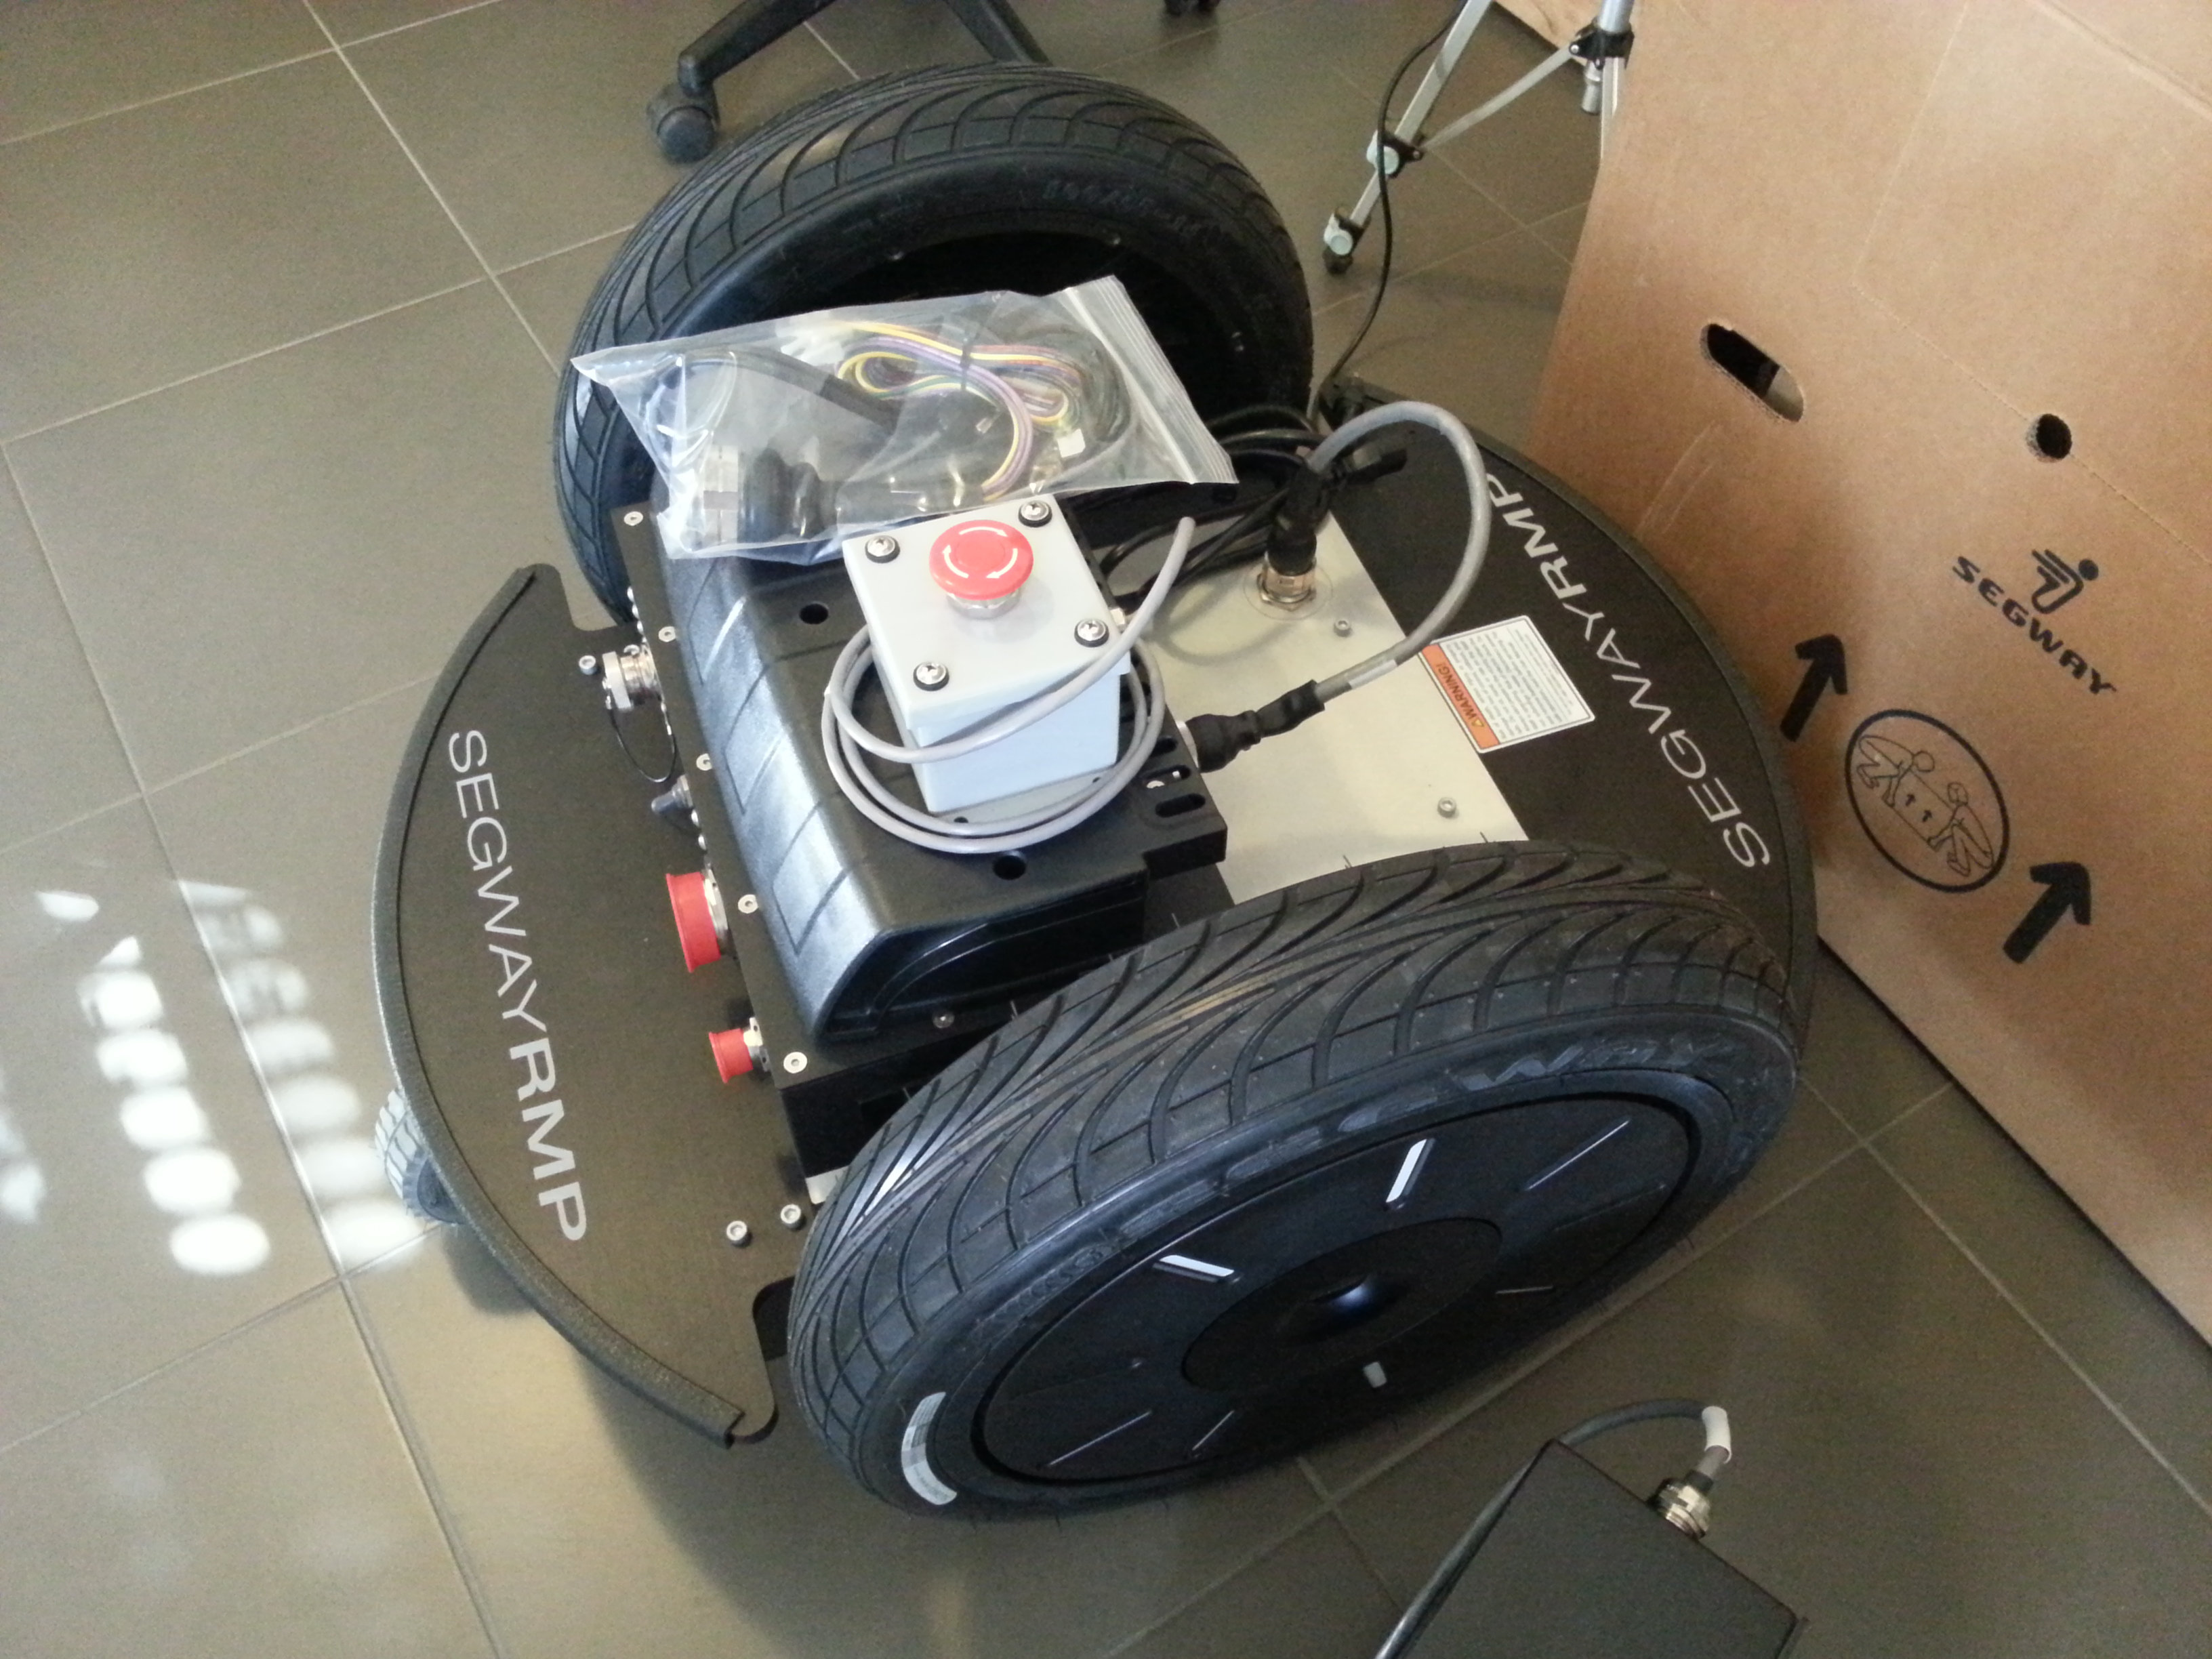
\includegraphics[height=5cm]{fig/segway_rmp210.jpg}
\end{center}
\caption{Segway RMP210 mobile platform.}
\label{fig:segway}
\end{figure}

\subsubsection{On-board sensors}

{\bf Laser range finders.} Two laser range finders equipped on the
front (Hokuyo UTM-30-LX) and back (Hokuyo URG-04LX-UG01) sides of the
robot will be used for robot localization, obstacle avoidance and
potentially people tracking.

Their specifications are summarized in the following table:

\begin{table}[h!]
\begin{tabular}{|c|c|c|}
\hline \bf{Model No.}& \bf{UTM-30-LX} & \bf{URG-04LX-UG01} \\
\hline \bf{Power source} & 12VDC±10\% & 5VDC±5\%(USB Bus power) \\
\hline \bf{Detection Range} & 0.1 to 30m (Max. 60m) & 20 to 5600mm \\
\hline \multirow{2}{*}{\bf{Accuracy}}
& 0.1 to 10m: $\pm$30mm  & 60 to 1,000mm: $\pm$30mm \\
& 10 to 30m: $\pm$50mm & 1,000 to 4,095mm: $\pm$3\% of measurement \\
\hline \bf{Scan Angle} & 270$^{\circ}$ & 240$^{\circ}$ \\
\hline \bf{Angular Resolution} & 0.25$^{\circ}$ & 0.36$^{\circ}$ \\
\hline \bf{Scan Time} & 25ms  & 100ms \\
\hline \bf{Weight} & Approx. 370g  & Approx. 160g \\
\hline
\end{tabular}
\caption{Hokuyo UTM-30-LX and URG-04LX-UG01 specifications.}
\end{table}

{\bf would be interesting to know which is the actual scanning angle due to the cover.}

\begin{figure}[h!]
\begin{center}
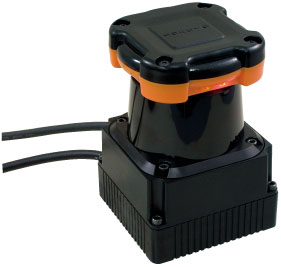
\includegraphics[height=4cm]{fig/utm30lx.jpg}
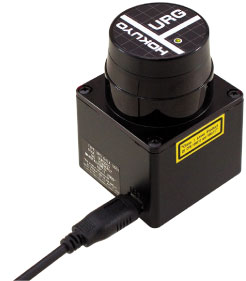
\includegraphics[height=4cm]{fig/urg04lxug01.jpg}
\end{center}
\caption{Hokuyo UTM-30-LX and URG-04LX-UG01 laser range finders.}
\label{fig:laserscans}
\end{figure}

{\bf Cameras.} The robot is mounted with 3 ASUS Xtion pro Live, a RGB
and Depth sensor that will be used for user gesture recognition,
people detection and tracking or detection of obstacles not visible by
the laser range finders. They will be arranged as it will be shown in
Section 3. 

Additionally, a Logitech HD Pro Webcam C920 is intended to be used for
robot localization in a later stage.  The camera will point to the ceiling
to take advantage of the special pattern (see Fig. \ref{fig:ceiling}) present in
the Rives de l'Orne mall, where the project demonstrations will be
carried out.

\begin{figure}[h!]
\begin{center}
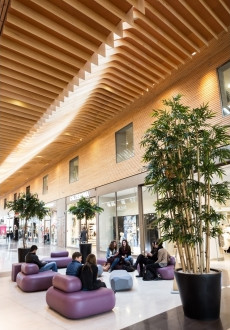
\includegraphics[height=4cm]{fig/ceiling.jpg}
\end{center}
\caption{Ceiling of the Rives de l'Orne shopping center.}
\label{fig:ceiling}
\end{figure}

\begin{figure}[h!]
\begin{center}
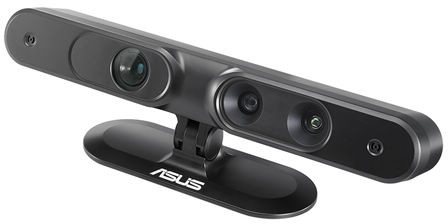
\includegraphics[height=4cm]{fig/asusxtionprolive.jpg}
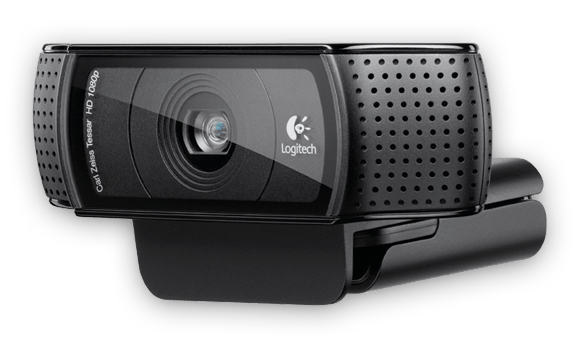
\includegraphics[height=4cm]{fig/logitech-hd-pro-webcam-c920.png}
\end{center}
\caption{ASUS Xtion pro Live and Logitech HD pro Webcam C920.}
\label{fig:cameras}
\end{figure}

\begin{table}[h!]
\begin{center}
\begin{tabular}{|c|c|}
\hline
& \bf{ASUS Xtion pro Live} \\
\hline \bf{ Power Consumption } & Below 2.5W \\
\hline \bf{ Distance of Use } & Between 0.8m and 3.5m \\
\hline \bf{ Field of View } & 58° H, 45° V, 70° D (Horizontal, Vertical, Diagonal) \\
\hline \multirow{2}{*}{\bf{ Depth Image Size }} 
& VGA (640x480) : 30 fps\\
& QVGA (320x240): 60 fps \\
\hline \bf{ Resolution } & SXGA (1280*1024)  \\
\hline \bf{ Interface } & USB 2.0 (USB 3.0 Ready) \\
\hline \bf{ Dimensions } & 18 cm x 3.5 cm x 5 cm \\
\hline
\end{tabular}
\end{center}
\caption{ASUS Xtion pro Live specifications.}
\end{table}

\begin{table}[h!]
\begin{center}
\begin{tabular}{|c|c|}
\hline
& \bf{Logitech HD Pro Webcam C920} \\
\hline \bf{Resolution } & Full HD video (up to 1920 x 1080 pixels) \\
\hline \bf{Video compression } & H.264 \\ 
\hline \bf{Interface } & USB 2.0 (USB 3.0 ready) \\
\hline \bf{Dimensions } & 29 mm x 24 mm x 24 mm \\ 
\hline \bf{Weight } & 162 g \\
\hline \multirow{2}{*}{\bf{Others}}
& Logitech Fluid Crystal™ Technology \\
& Carl Zeiss lens with 20-step autofocus \\
& Automatic low-light correction \\
\hline
\end{tabular}
\end{center}
\caption{Logitech HD Pro Webcam C920 specifications.}
\end{table}

\subsubsection{Human-Robot Interfaces}
Interaction with the user will be mainly through a Graphical User
Interface (GUI) displayed on a tablet Microsoft Surface Pro 2.
Although this device already incorporates stereo speakers and a
microphone, additional built-in speakers are mounted on the robot
structure and an external microphone will be used to receive commands
and spoken requests from the user. Concretely, a RODE NTG-2
professional microphone has been chosen for its capability to
eliminate the surrounding noise and focus audio recording from the main direction it is pointing to
as it is shown in Fig. \ref{fig:microphone}.
Below, we describe the main technical specifications of these devices.

\begin{table}[h!]
\begin{center}
\begin{tabular}{|c|c|}
\hline
& \bf{Microsoft Surface Pro 2} \\
\hline \bf{Software} & Windows 8.1 Pro \\
\hline \bf{Dimensions} & 27.46 cm x 17.30 cm x 1.35 cm \\
\hline \bf{Weight} & 907g \\
\hline \bf{Storage} &  64/128GB/256/512GB \\
\hline \bf{Memory} & 4GB RAM  /    8GB RAM \\
\hline \multirow{3}{*}{\bf{Display}}
& Screen: 10.6 inch ClearType Full HD Display \\
& Resolution: 1920 x 1080 \\
& Touch: 10-point multi-touch \\
\hline \bf{CPU}  & 4th generation Intel\textsuperscript{\textregistered} Core\textsuperscript{TM} i5 Processor \\
\hline \multirow{2}{*}{\bf{Wireless Connections}} 
& Wireless: Wi-Fi (802.11a/b/g/n) \\
& Bluetooth 4.0 Low Energy technology \\
\hline \multirow{2}{*}{\bf{Camera, Video \& Audio}}  
& Two 720p HD cameras, front and rear-facing \\
& Microphone and Stereo speakers \\
\hline \multirow{3}{*}{\bf{Ports}} 
& Full-size USB 3.0 \\
& microSDXC card reader \\
& Headset jack \\
\hline \multirow{4}{*}{\bf{Sensors}}
& Ambient light sensor \\
& Accelerometer \\
& Gyroscope \\
& Magnetometer \\
\hline
\end{tabular}
\end{center}
\caption{Microsoft Surface Pro 2 specifications.}
\end{table}

\begin{table}[h!]
\begin{center}
\begin{tabular}{|c|c|}
\hline
& \bf{Microphone RODE NTG-2} \\
\hline \bf{Acoustic Principle } & Line plus gradient \\
\hline \bf{Directional Pattern } & Super-Cardioid (see Fig. \ref{fig:microphone}) \\
\hline \bf{Frequency Range } & 20Hz ~ 20kHz selectable \\
\hline \bf{Output Impedence } & 250$\Omega$ \\
\hline \bf{Maximum SPL } & 131dB (@ 1kHz, 1\% THD into 1k$\Omega$ load) \\
\hline \bf{Maximum Output Level } & 6.9mV \\
\hline \multirow{2}{*}{\bf{Sensitivity}} 
& -36dB re 1 Volt/Pascal (15mV @ 94dB SPL) \\
& $\pm$2dB @ 1kHz \\
\hline \bf{Equivalent Noise } & 18dB-A SPL \\
\hline \bf{Power Requirement } & Phantom P48 or 1.5V Alkaline ‘AA’ Battery \\
\hline \bf{Output Connection } & 3-pin XLR Output \\
\hline \bf{Dimensions } & 280 mm x 22 mm x 22 mm \\
\hline \bf{Net Weight } & 161g \\
\hline
\end{tabular}
\end{center}
\caption{Microphone RODE NTG-2 specifications.}
\end{table}

\begin{figure}[h!]
\begin{center}
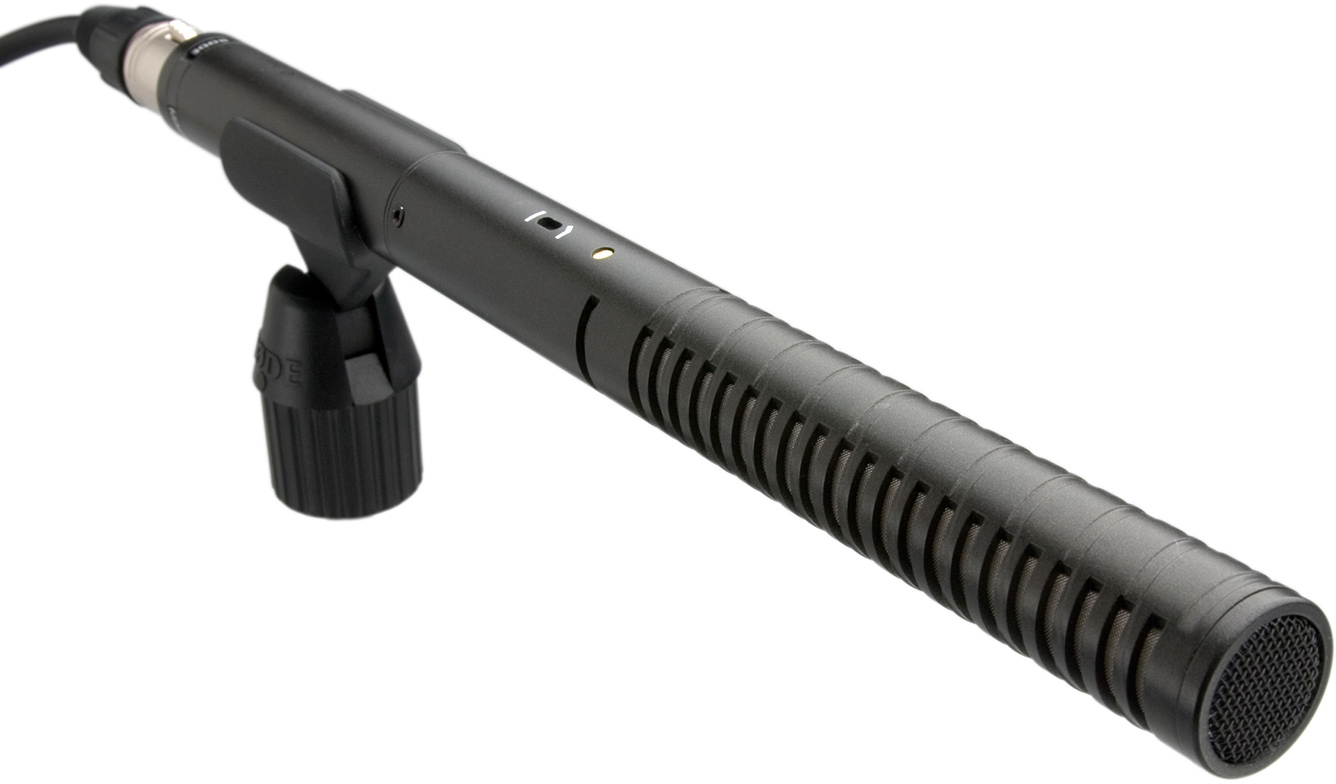
\includegraphics[height=4cm]{fig/ntg2.jpg}
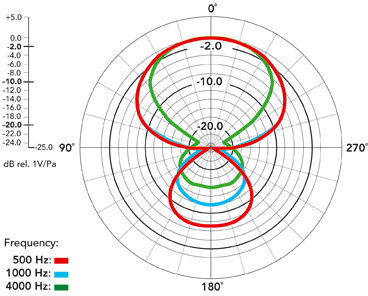
\includegraphics[height=4cm]{fig/ntg2polar.jpg}
\end{center}
\caption{Microphone RODE NTG-2 and polar pattern.}
\label{fig:microphone}
\end{figure}



\subsubsection{Additional devices}
The robot platform, sensors and human-robot interfaces described above will be connected
through a PC laptop and 3 Odroid C1 Single Board Computers (SBC) (see Fig. \ref{fig:odroid}) that will free the main computer from processing load.
A network switch will interconnect all these devices and will provide internal communication as well as external wireless access to the communication network installed in the building.
The technical specifications of the laptop, a HP EliteBook 820 G2, and of the Odroid C1 boards are presented below.
The arrangement of all the devices on the robot will be explained in the next section.


\begin{table}[h!]
\begin{center}
\begin{tabular}{|c|c|}
\hline
& \bf{HP EliteBook 820 G2} \\
\hline \bf{Operating system } & Ubuntu Linux \\
\hline \bf{Processor} & Intel\textsuperscript{\textregistered} Core\textsuperscript{TM} i3-5010U (2.1GHz, 3MB L3 Cache) \\
\hline \bf{Memory} & \\
\hline \bf{Internal Storage} & \\
\hline \bf{Graphics} & Intel\textsuperscript{\textregistered} HD Graphics 5500 \\
\hline \bf{Dimensions } & 31 cm x 21.5 cm x 2.1 cm \\
\hline
\end{tabular}
\end{center}
\caption{Specifications of the HP EliteBook 820 G2.}
\end{table}

\begin{table}[h!]
\begin{center}
\begin{tabular}{|c|c|}
\hline
& \bf{ODROID-C1} \\
\hline \multirow{3}{*}{\bf{CPU }}	
& Amlogic S805 SoC  \\
& 4 x ARM\textsuperscript{\textregistered} Cortex\textsuperscript{\textregistered}-A5 1.5GHz \\
& ARMv7 Architecture @28nm \\
\hline \bf{GPU } & 2 x ARM\textsuperscript{\textregistered} Mali\textsuperscript{TM}-450MP 600MHz \\
\hline \bf{RAM } & 1GB 32bit DDR3 792MHz \\
\hline \bf{Flash Storage } &	Micro-SD UHS-1@100Mhz/SDR50 or eMMC storage option \\
\hline \bf{USB2.0 Host } & 4 Ports \\
\hline \bf{USB2.0 Device / OTG } & 1 Port for Linux USB Gadget driver \\
\hline \bf{Ethernet/LAN } & 10/100/1000 Mbit/s \\
\hline \bf{Video and Audio Output } & HDMI \\
\hline \bf{Camera Input } & USB 720p \\
\hline \bf{Size } & 85 mm x 56 mm \\
\hline \bf{Weight } & 40 g \\
\hline
\end{tabular}
\end{center}
\caption{Specifications of the ODROID-C1 board.}
\end{table}

\begin{figure}[h!]
\begin{center}
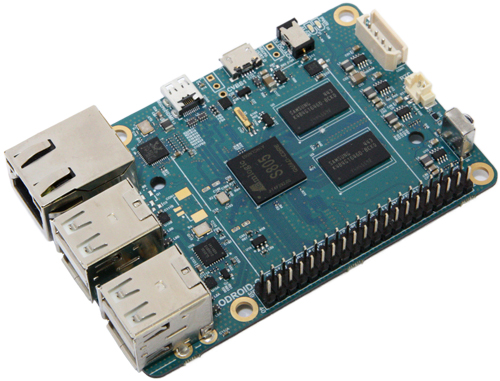
\includegraphics[height=4cm]{fig/odroidc1.jpg}
\end{center}
\caption{Odroid C1 board.}
\label{fig:odroid}
\end{figure}

\subsection{Device Connections}
All the devices presented in the previous section are integrated in
the robot as shown in Fig. \ref{fig:architecture}.

The main functionalities and behaviour of the robot will be managed by
the laptop which will run the ROS master under Linux to synchronize the different
modules of the system.  However, we propose a balanced architecture
where the sensor data acquisition and its subsequent processing is not
handled by this single computer.  Instead, cameras, laser range
finders as well as the robotic platform are connected via USB to the 3
Odroid boards which will be in charge of the acquisition and
processing tasks. In particular, the data acquisition from the ASUS
Xtion cameras is the most expensive in terms of processing
requirements. Consequently, this process is distributed by connecting
the cameras into the 3 different Odroid boards.

The data transfer between the SBCs, the laptop and the human-robot
interfaces will be through Ethernet connection using the network
switch. This component will also provide the system with wireless access to external
devices such as the cameras placed in the building or to the communication infrastructure.

Buiding such distributed system offers one additional advantage, among others. 
Device drivers can be installed on the SBCs to maintain a stable interface with the hardware, 
independent of the particular configuration of the main laptop, its operating system or its kernel version.
Next section will describe the specific device drivers that will be used in the robot set-up.

\begin{figure}[h!]
\begin{center}
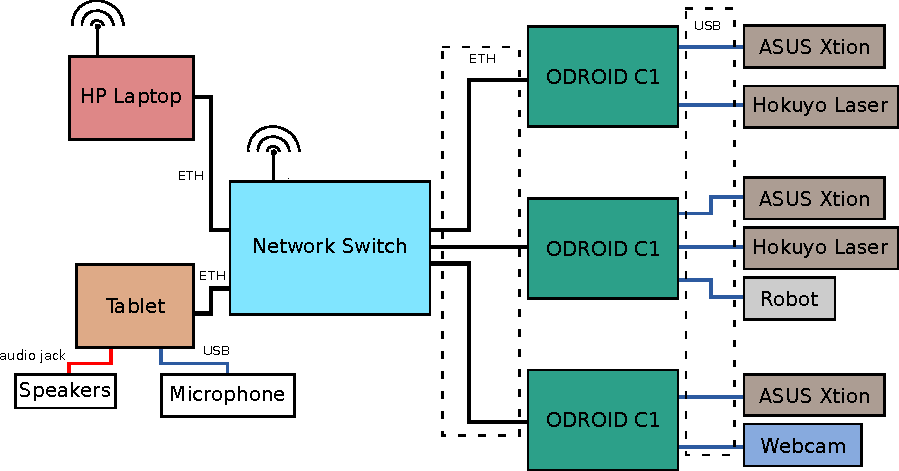
\includegraphics[height=6cm]{fig/robotarchitecture.pdf}
\end{center}
\caption{Robot Architecture.}
\label{fig:architecture}
\end{figure}


\subsection{Device drivers}

Device drivers provide a communication interface between the hardware
components and the operating system. Most of the drivers for the
robotic devices are publicly available through the ROS
community. However, they lack of uniformity and produce a lot of
complex information that is not always necessary for certain
applications. Additionally, we encountered some issues when running
these drivers on embedded boards.

For these reasons, at Sapienza University we started to develop
\textit{thin\_drivers}\footnote{https://github.com/grisetti/thin\_drivers},
our own suite of lightweight device drivers.

They provide a unified ROS interface for the most common devices such
as RGB-D cameras (e.g., ASUS Xtion), laser scanners (e.g., the Hokuyo
family) or IMUs. The drivers are minimal, in the sense that they
publish only a subset of the information produced by the sensor and
can be modified based on the user needs.







\section{Communication Infrastructure}

general overview od communication infrastructures for robot-robot and robot-external device communicatins....


\subsection{TCP Interface}








\section{Robot Design}

The design of the COACHES robots has been carried out within a study made by
the designer Roberto Tino\footnote{www.robertotino.com}, during a collaboration
with Dept. of Computer, Control and Management Engineering Sapienza University of Rome, Italy.


The designed robot model has been called ALFRED and the main design concept has been developed for the need of deploying a social robot in public environments (such as, shopping malls) with the purpose of assisting people that need for help or
information, guiding them to a certain location, etc.

The main results of the design are reported in the following of this section.


\subsection{Motivation and design goals}

In previous years, robots were mostly used within
factories or non-public spaces and thus their look was not
a crucial aspect. The essential thing for a good robot was
to carry out its programmed job in a precise and
repetitive manner. Its shape was designed mainly for
functionality and the interaction with humans was limited
to technicians instructed on how to use them.
Recently, more and more robotic applications have
moved into public space populated by non-expert users.
Consequently, robot appearance started to evolve to adapt
to the public and domestic environments and forms of
natural interactions with users (e.g., speech) are emerging
thanks also to the developments in the field of artificial
intelligence.

Finally, many studies on social robotics require to design and realize robots that can operate in very close
contact with people and can perform in general social acceptable behaviors. The shape of this kind of robots
has a fundamental role; it has to suggest the interaction and to raise the people curiosity. The appearance has
to be friendly and has not to instill dread.

Following this trend, we have designed and developed a social robot for public environment, as described in
the following of this abstract. The design has followed guidelines and use cases of the COACHES project,
that aims at developing autonomous social robots operating in a shopping mall in Caen, France and
performing short-term interactions with shop-keepers and customers of the mall.
Moreover, given the actual goal of fully producing two of these robots to be deployed in a real shopping
mall, architectural and functional limits derived by limited budget have been carefully considered.
The two robots are under development from Algorithmica S.r.l.\footnote{http://algorithmica.it} company and they are expected to be delivered in Fall 2015.

\subsection{Design concepts}

ALFRED is a social robot designed to operate in public environments populated by many non-expert users.
Its main purpose is to assist people that ask for help or information, need to be guided to a certain
location, as well as to advertise items and goods as provided by shop-keepers.
As being in front of something that looks human but is not human can instill dread to the user, we chose not
to use an anthropomorphic shape for the robot.

However, size and shape of the robot resemble those of a human. In this way we expect the robot to suggest
natural human-like interactions (such as, using speech or gestures). The structure is erect and curved ahead to
have a servile aspect and it is not taller than a human.

One main objective of this design was to create a robust and light robot that can stimulate interactions from
users.
The robotic base guarantees a very smooth and agile motion in indoor environments, sensors and
computational power allows for realizing complex behaviors and multi-modal interactions, while the carbon
structure provides robustness and lightness.
The molded components design is very minimal and it is composed of simple shapes, like spheres or
triangles, the surfaces are smooth and accommodating without corners or sharp edges.

The result of the design is illustrated in the following figures.

\begin{center}
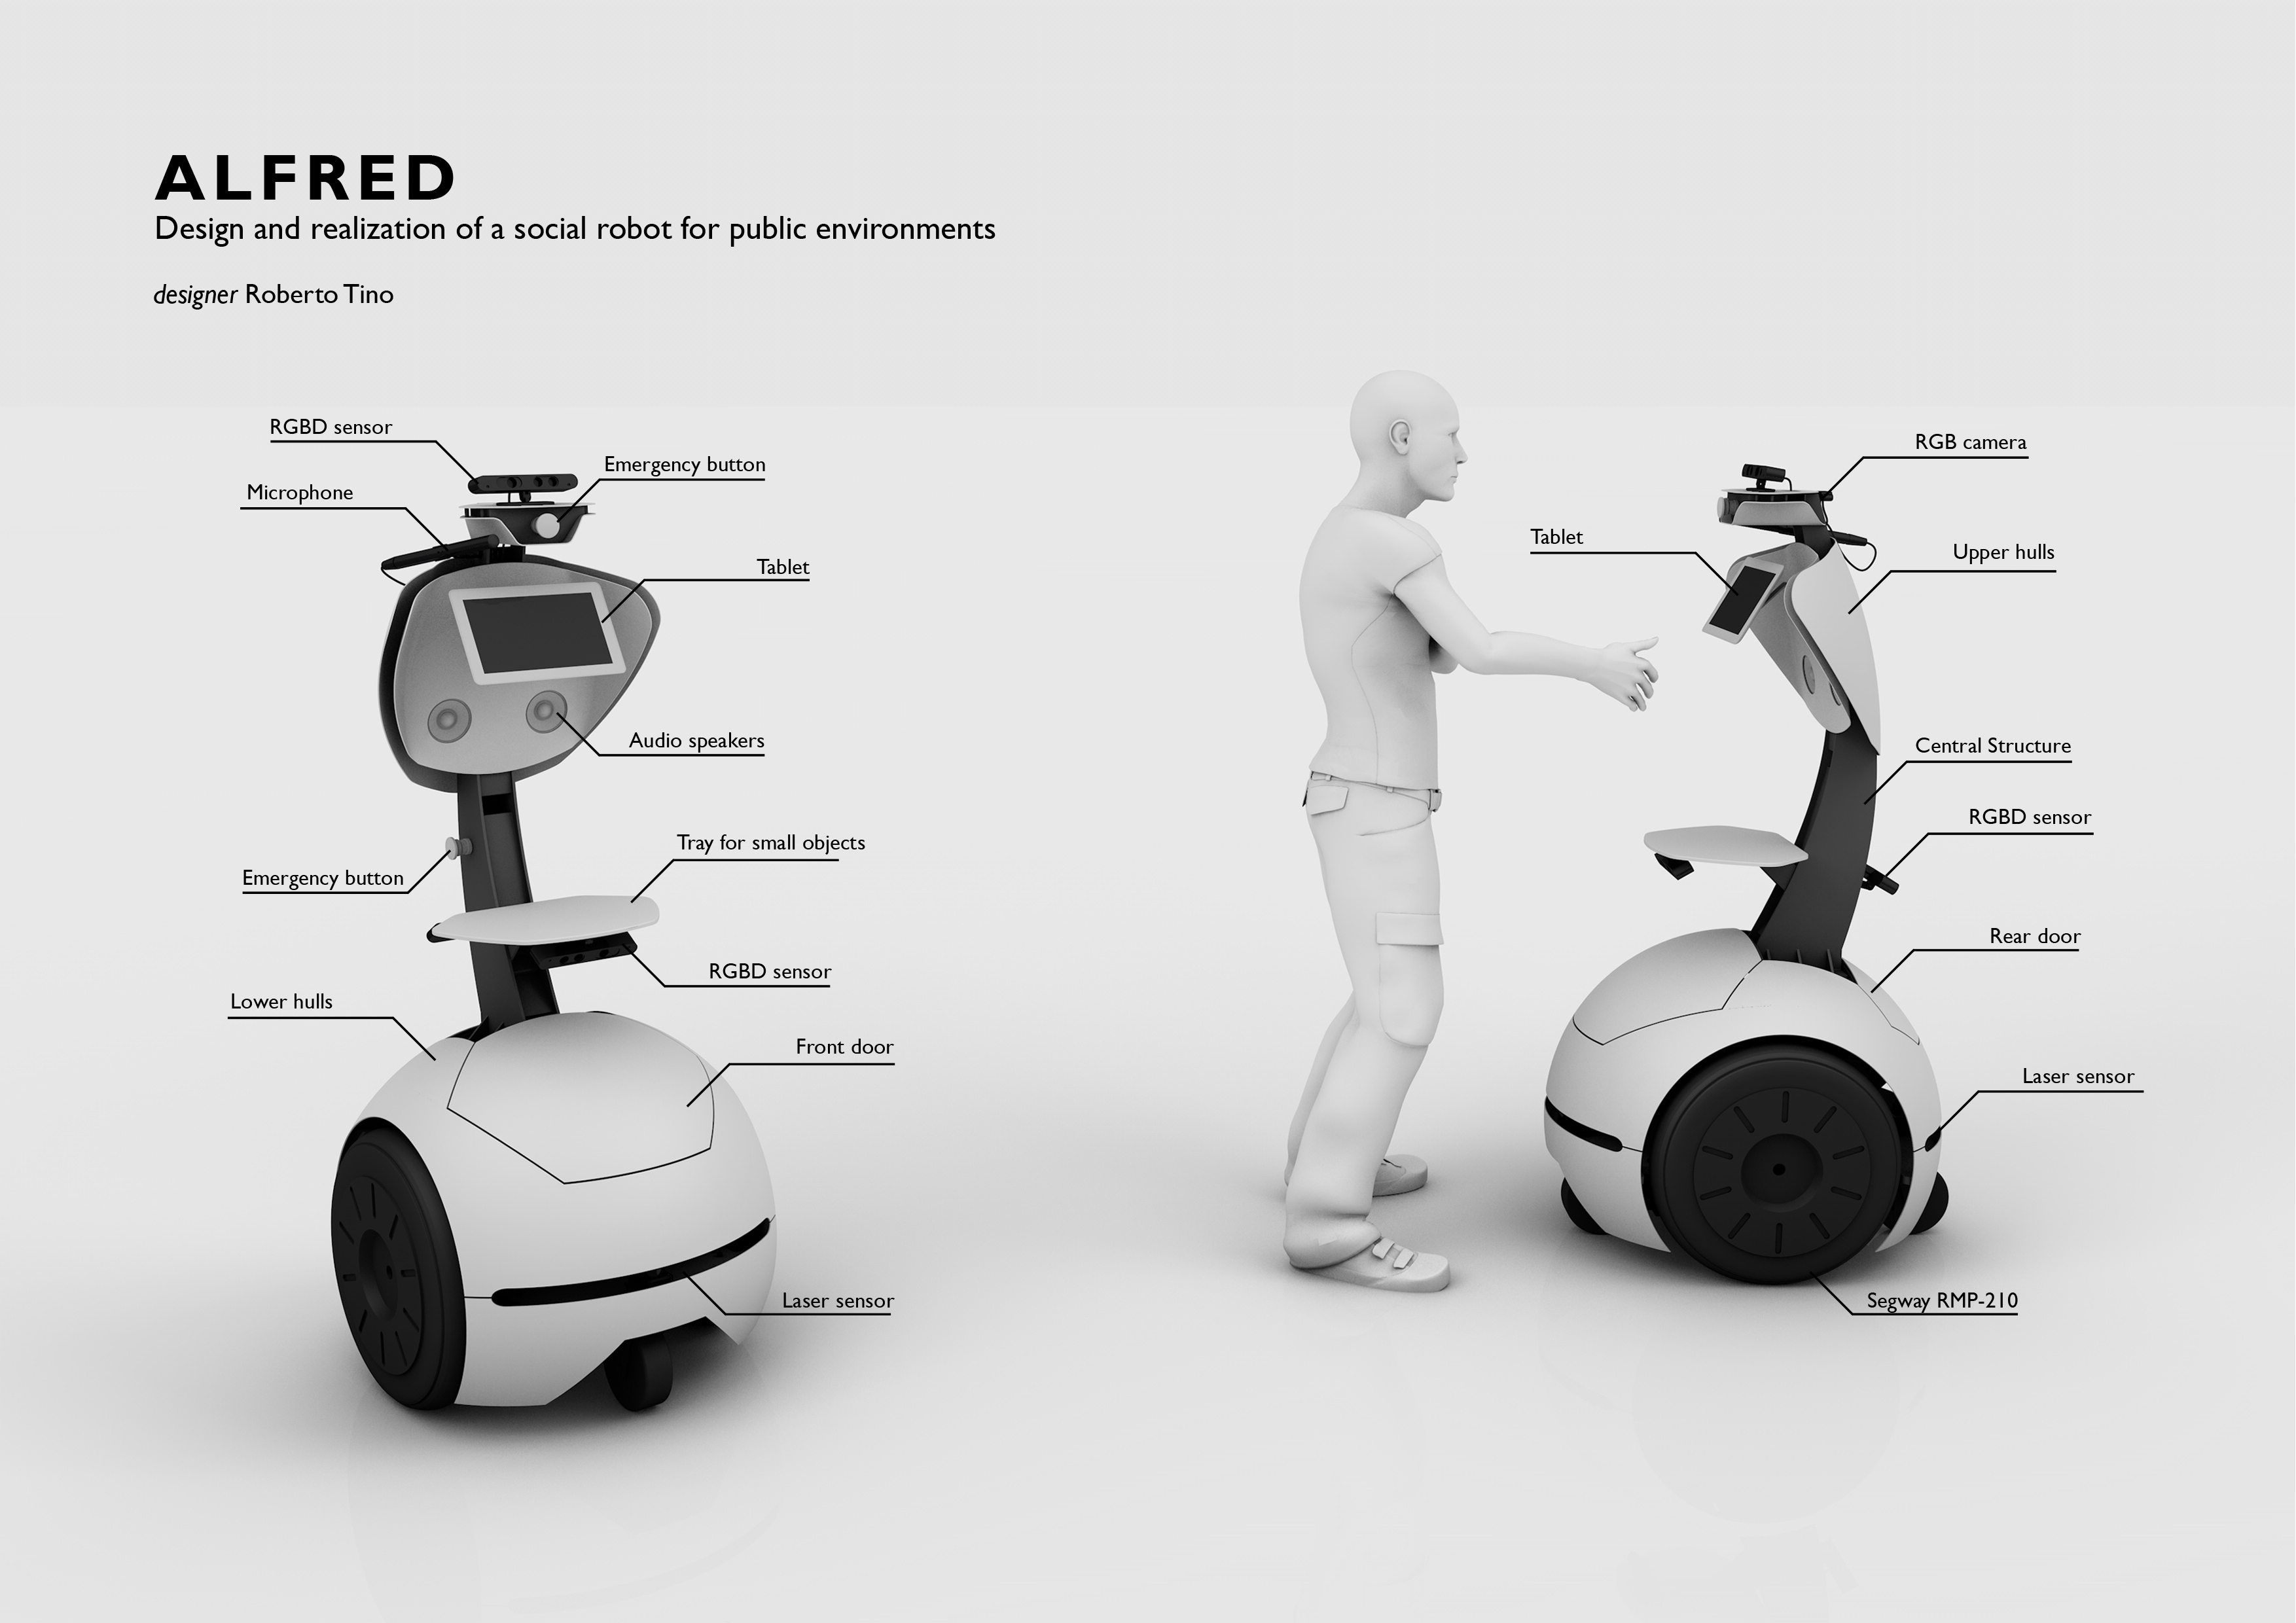
\includegraphics[height=10cm]{fig/Tavola01.jpg}
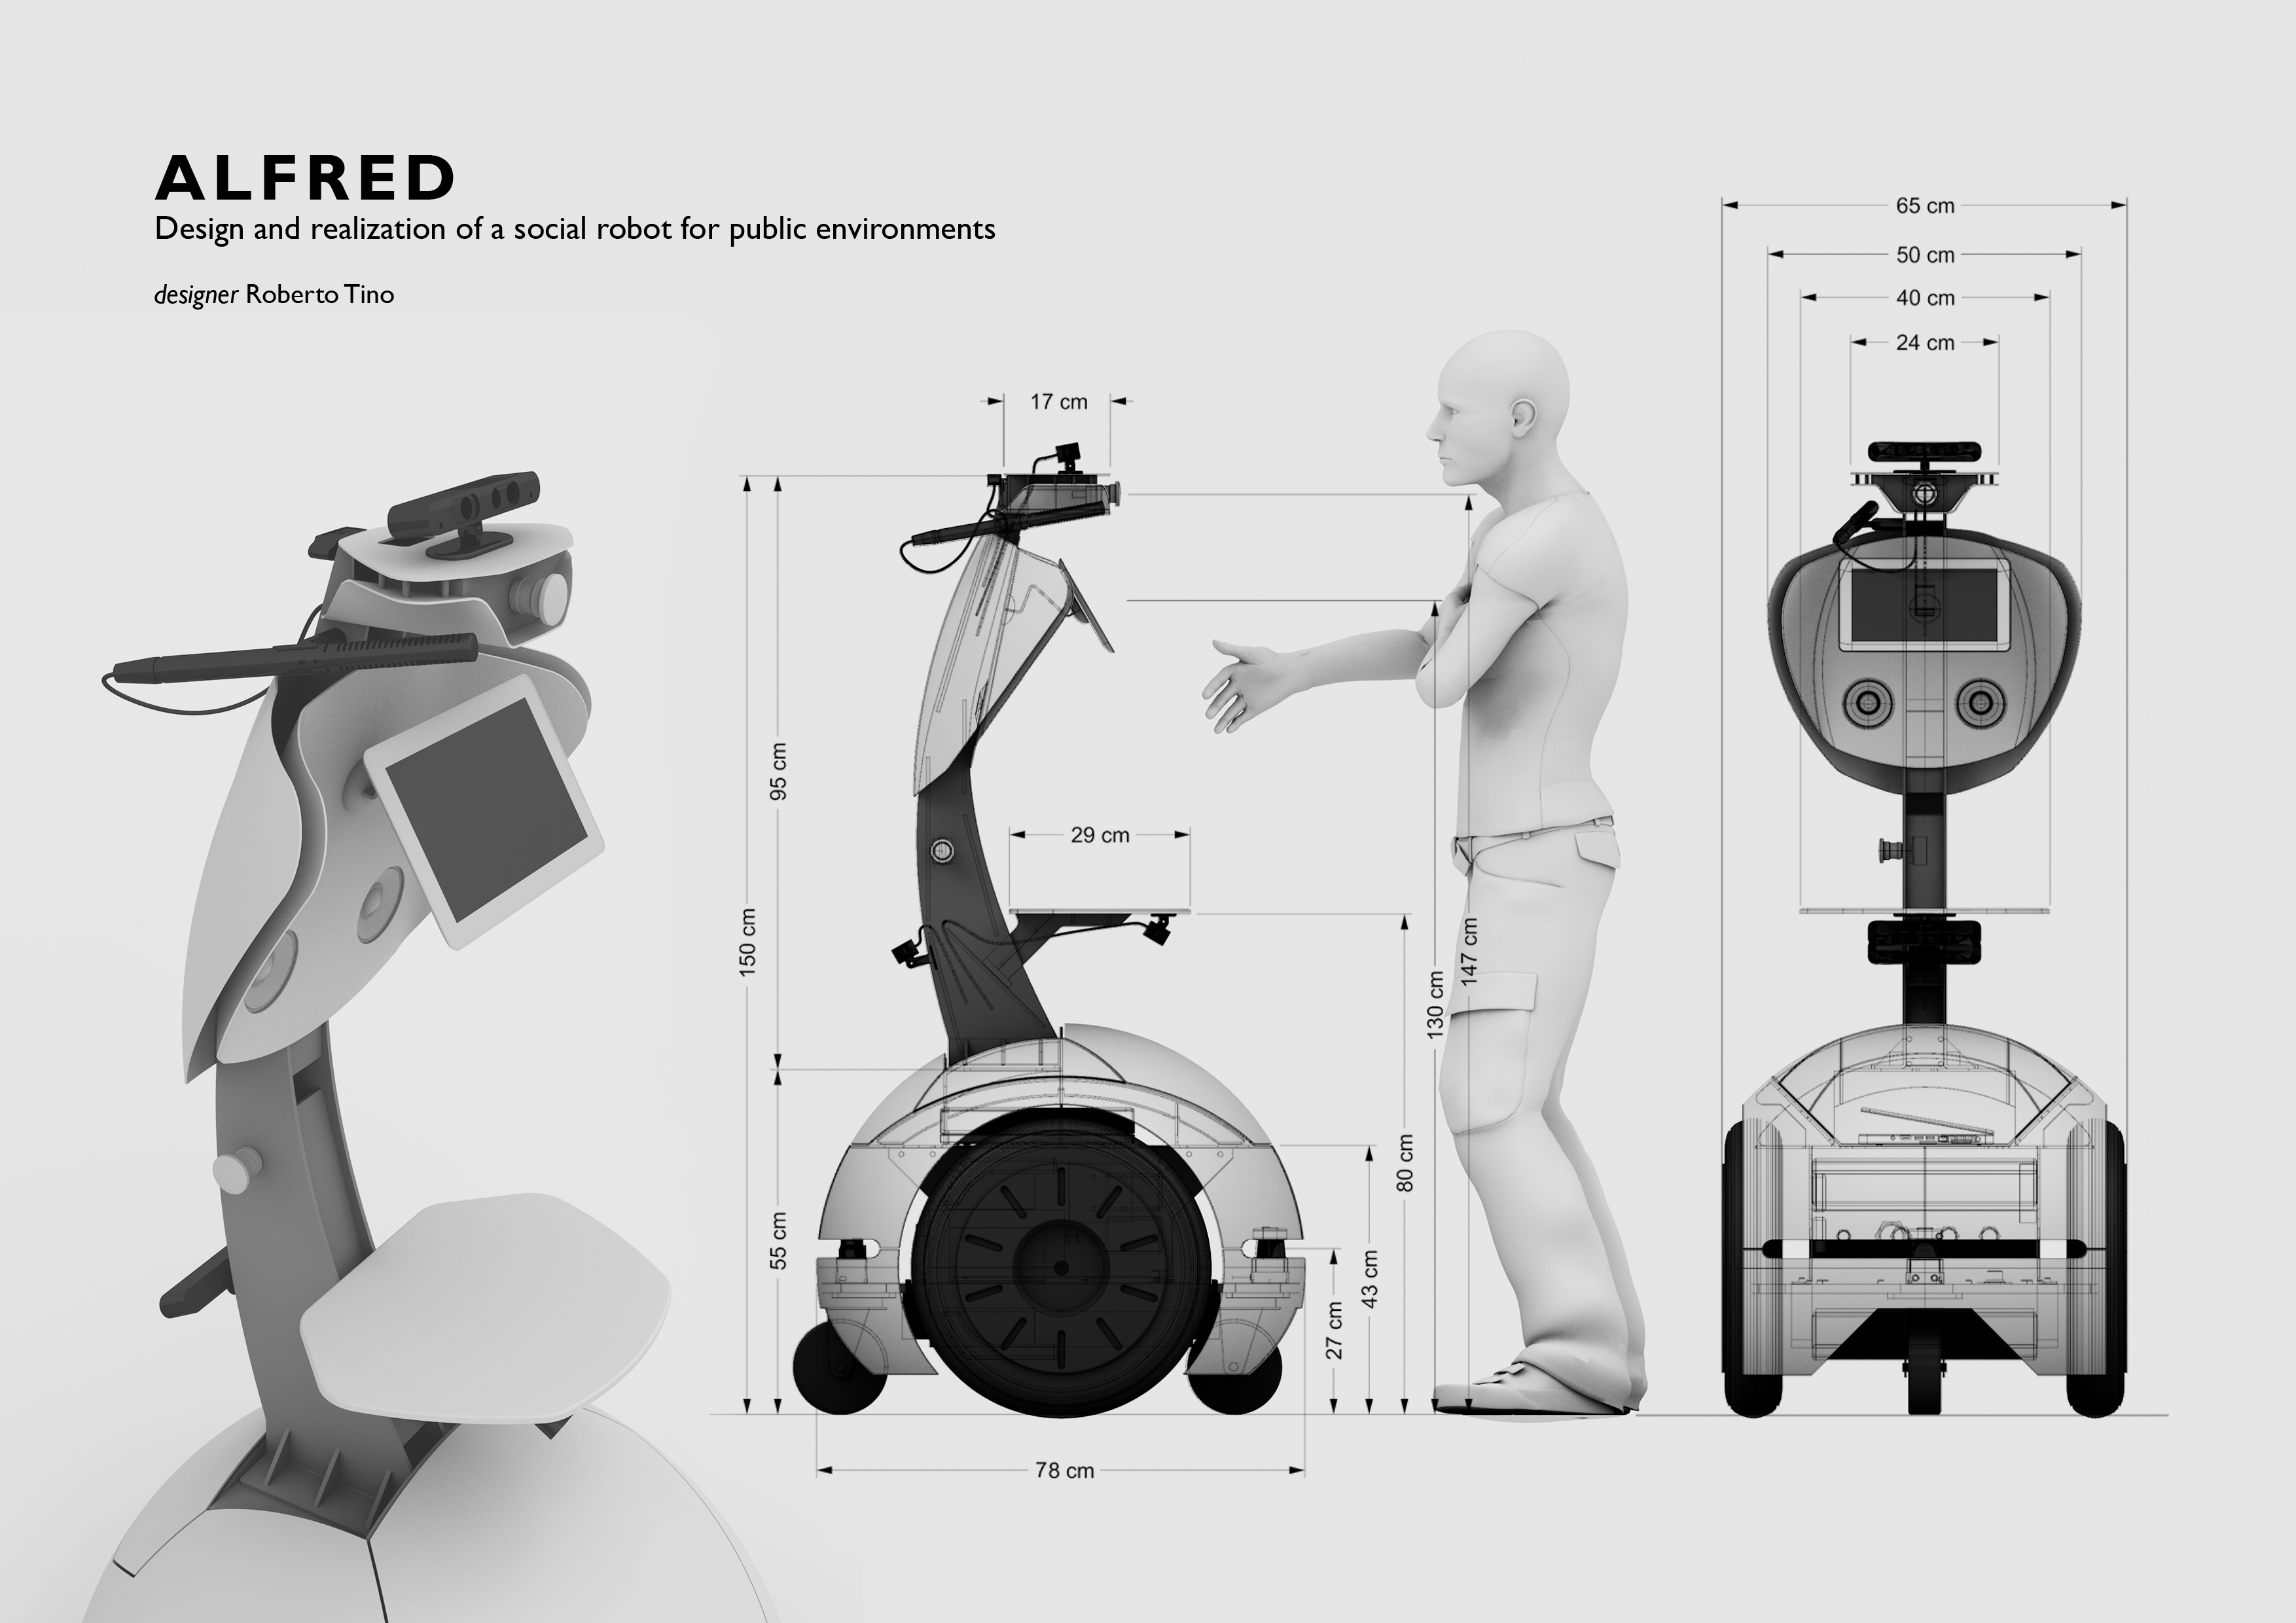
\includegraphics[height=10cm]{fig/Tavola02.jpg}
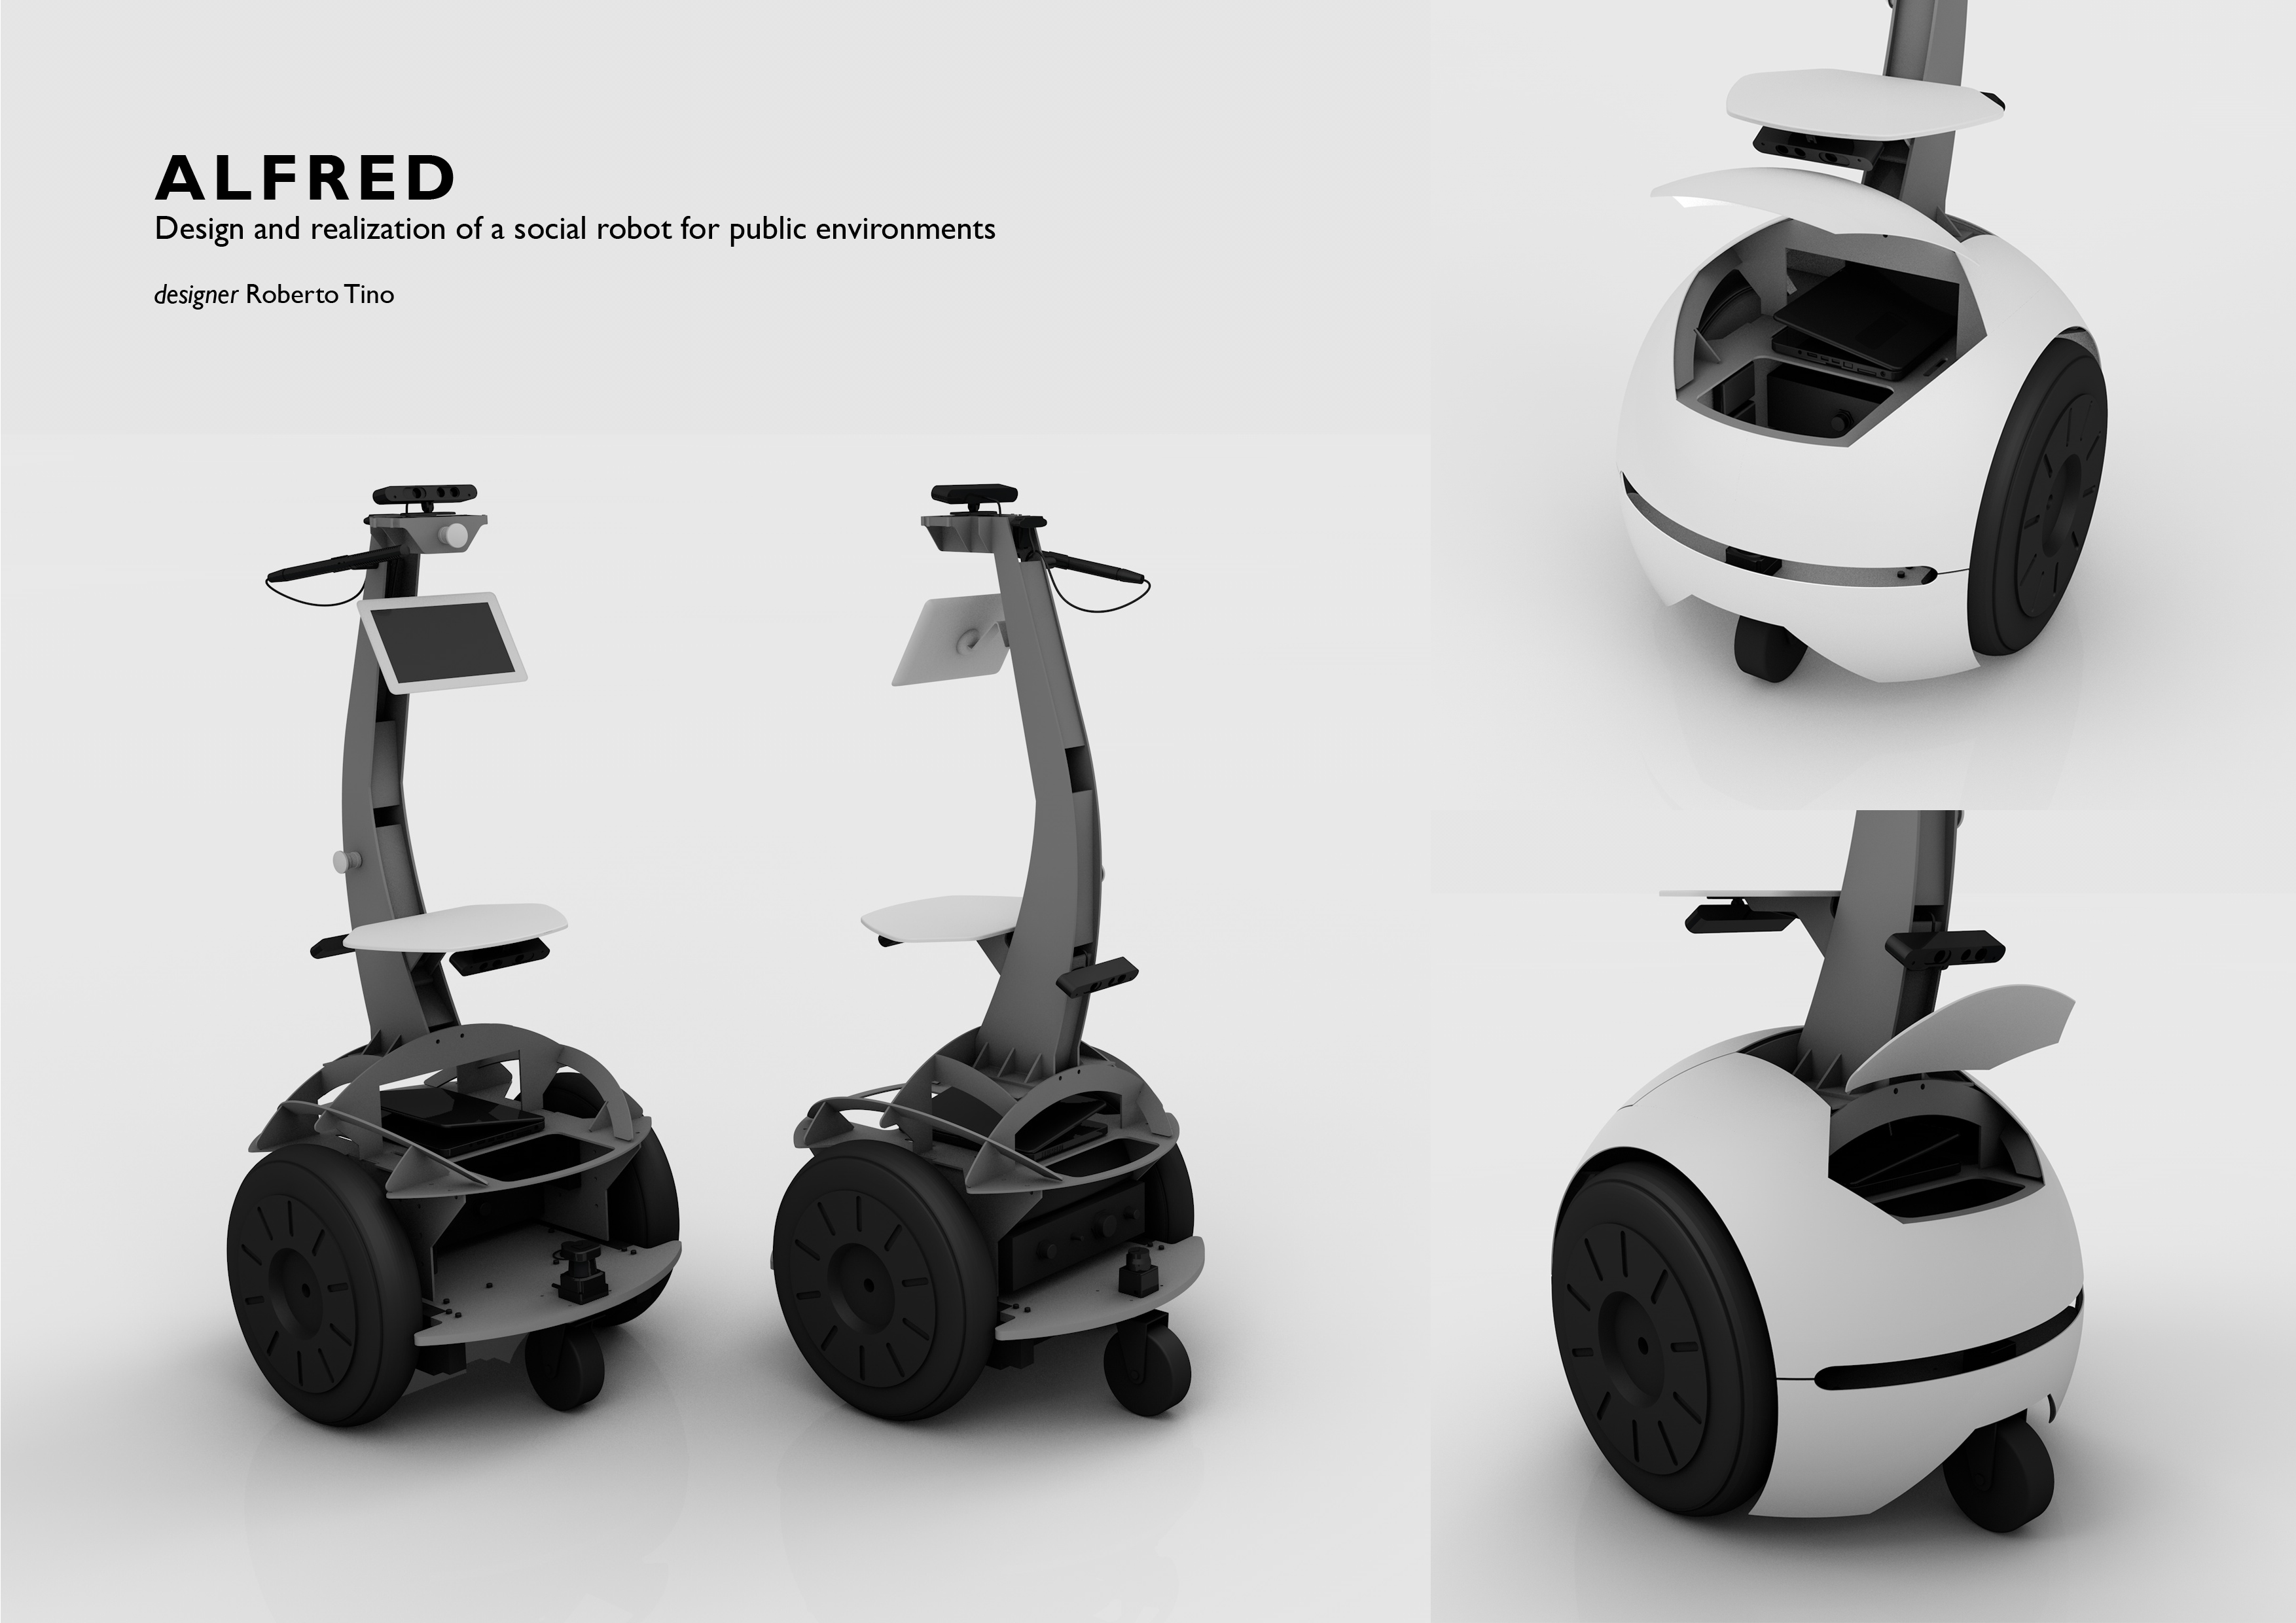
\includegraphics[height=10cm]{fig/Tavola03.jpg}
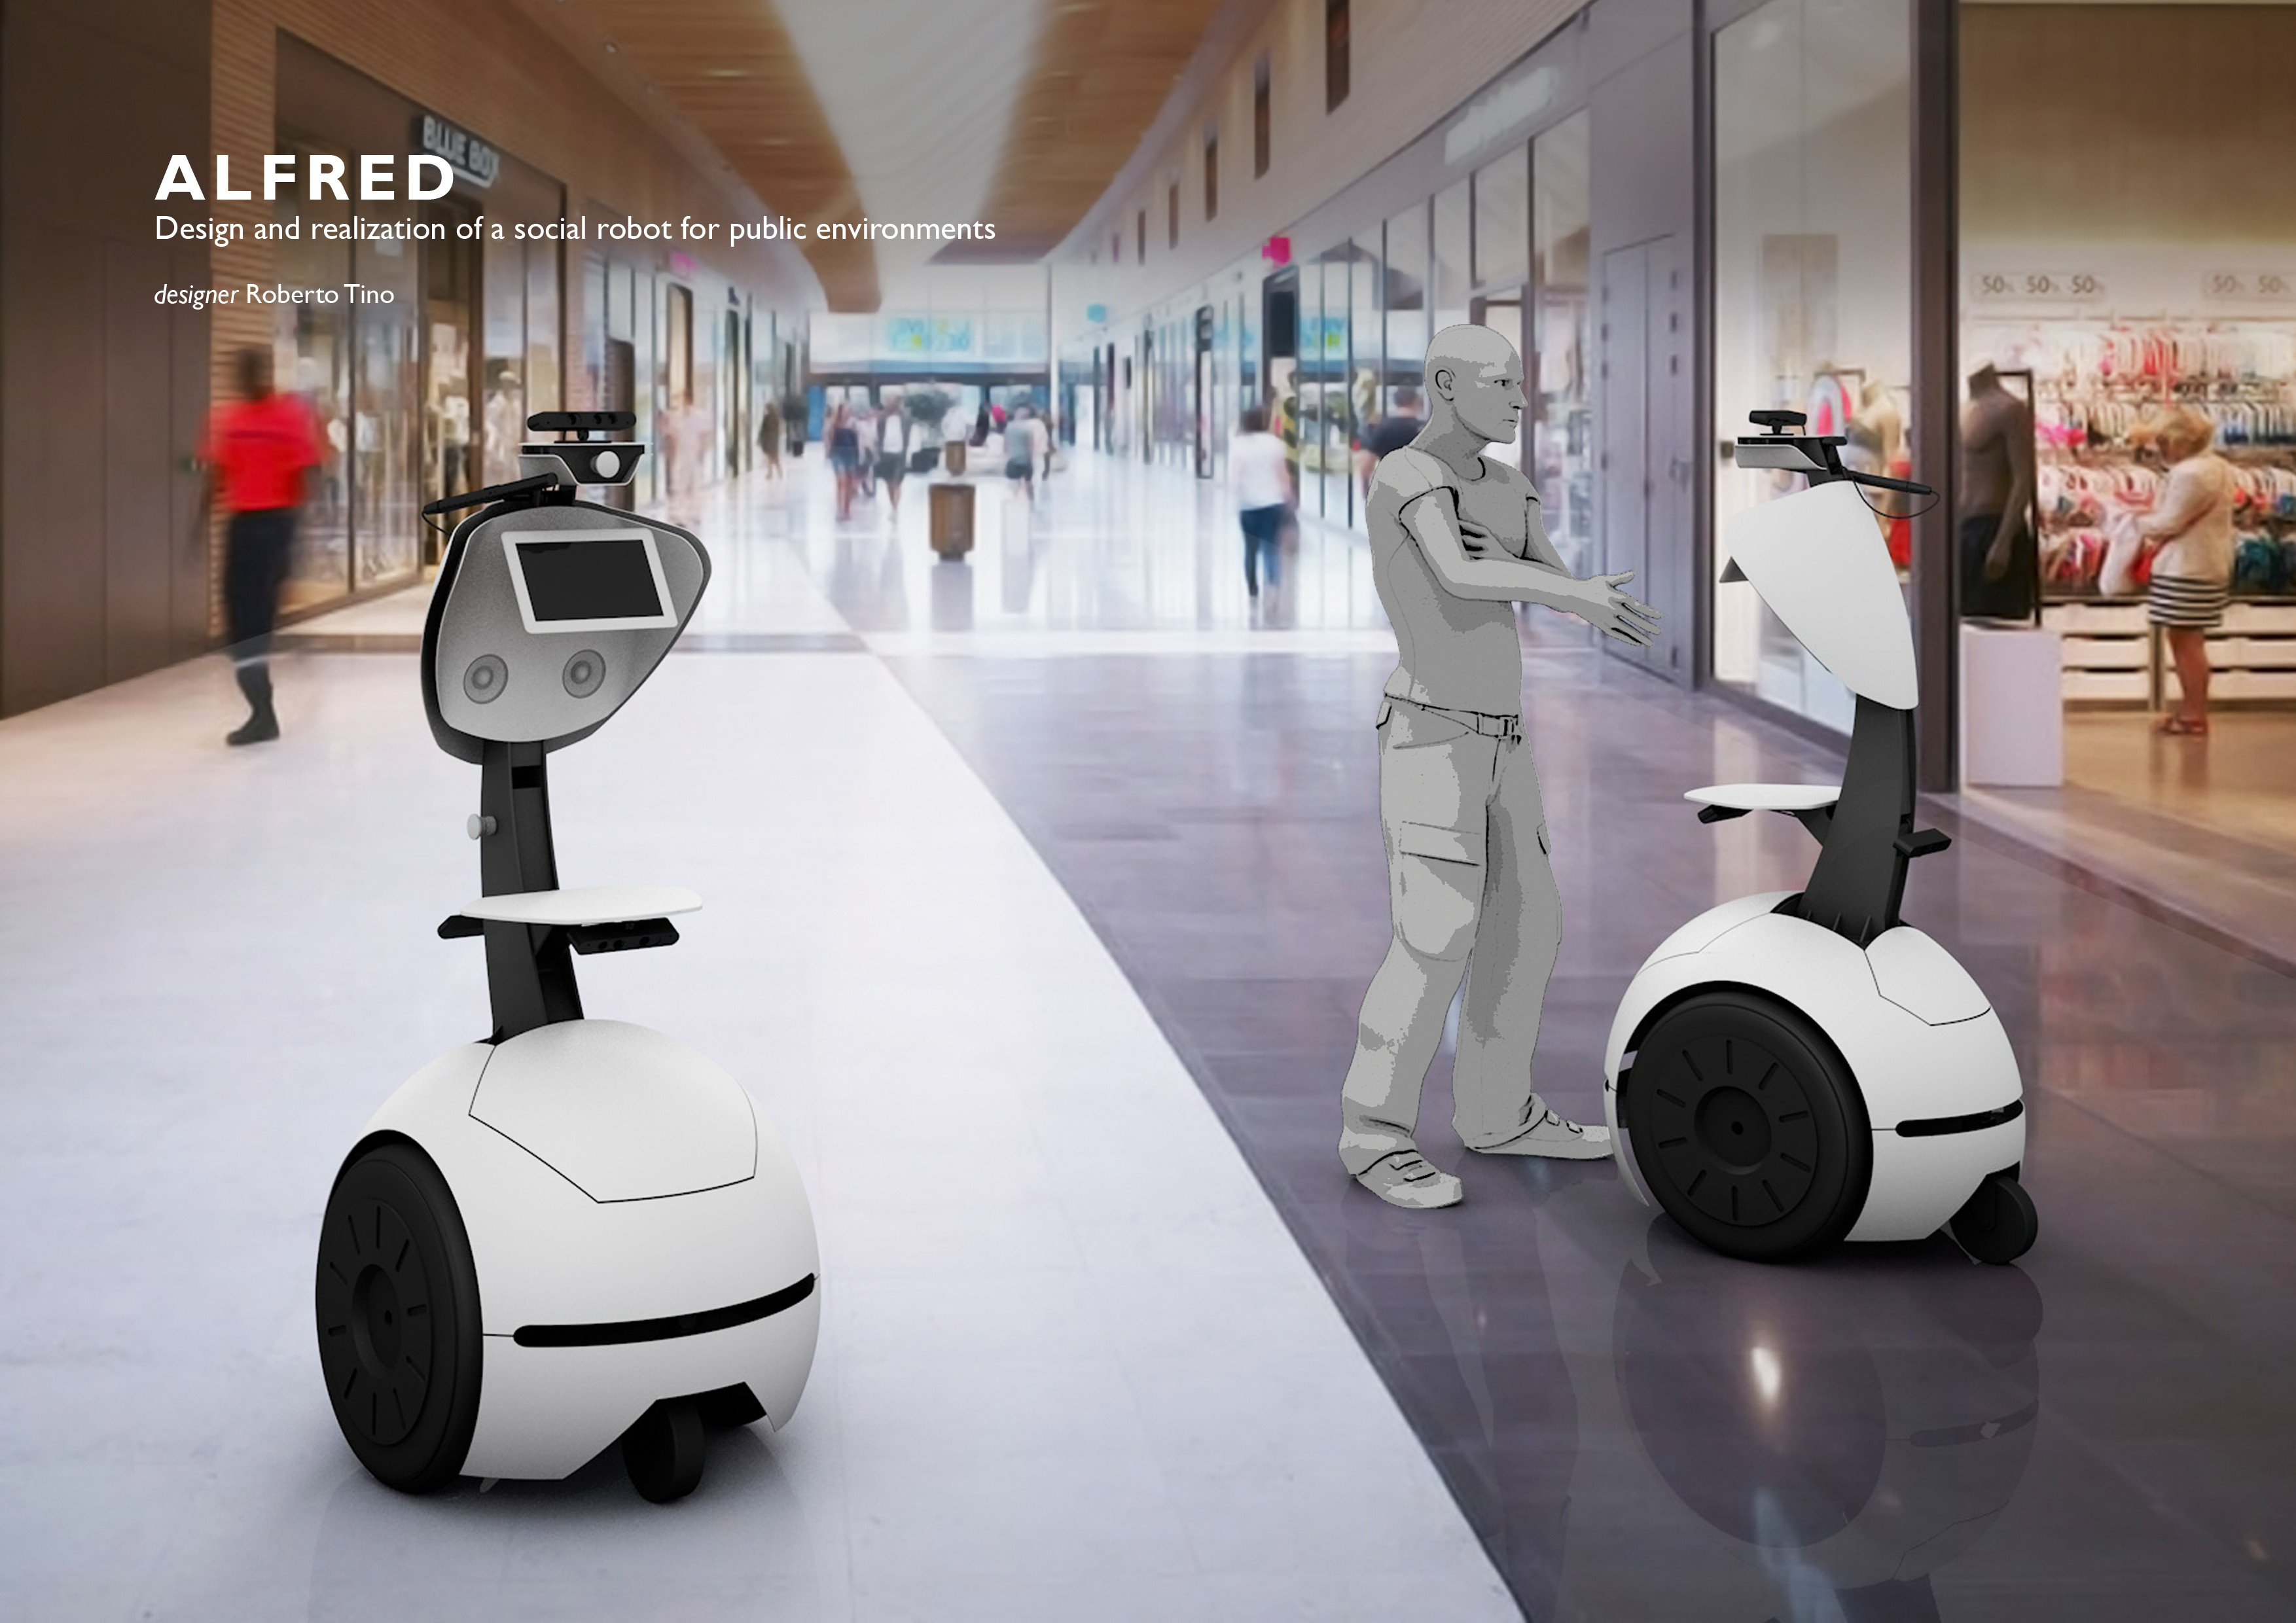
\includegraphics[height=10cm]{fig/Tavola04.jpg}
\end{center}


\subsection{Realization}

The robot is built using a Segway robotic base RMP-210 and it is composed by a central carbon structure
obtained from flat plates that are later dovetailed and glued with each other.
The robot lower casing is designed to host a laptop, two laser sensors and all the electronic needed to control
the robot, while the top partis a sort of backbone that housestwo or three RGBD sensors, a camera, a tablet,
two audio speakers, the microphone and a tray where to place small objects.
External hulls are arranged upon the main structure with the purpose of protecting the components and to
give a pleasant look. The hulls are made of a composite material, laminated on mold previously created.
Finally, the two parts of the robot are easy to disassemblefor transportation.





\end{document}
